\documentclass{article}
\usepackage{color}
\usepackage{graphicx}
\usepackage{amsmath}
\usepackage{enumerate}
\usepackage{bm}
\usepackage{footnote}
\usepackage{enumerate}
\usepackage{booktabs}
\usepackage{cite}
\usepackage{geometry}
\usepackage[marginal]{footmisc}
\usepackage{url}
\usepackage{float}
\usepackage{indentfirst}
\usepackage{ulem}
\usepackage[colorlinks,linkcolor=black]{hyperref}
\usepackage{multirow}
\usepackage{amssymb}
\usepackage{cite}
\usepackage{makecell,rotating,multirow,diagbox}
\setlength{\parindent}{14pt}
\setlength{\parskip}{12pt plus1pt minus1pt}

%\documentclass[a4paper]{article}
\usepackage{amsmath,graphicx,geometry,booktabs,epstopdf,wrapfig,setspace,colortbl,color,subfigure,indentfirst,multirow,float}
\usepackage[version=4]{mhchem}
\usepackage{tikz}
\usepackage{etoolbox}
\usepackage{enumitem}
\newcommand*{\circled}[1]{\lower.7ex\hbox{\tikz\draw (0pt, 0pt)%
    circle (.5em) node {\makebox[1em][c]{\small #1}};}}
\robustify{\circled}
\geometry{a4paper,left=2.54cm,right=2.54cm,top=2.54cm,bottom=2.54cm}
\renewcommand\thesection{\Roman{section}}
\renewcommand\thesubsection{\indent{\Alph{subsection}}}
\begin{document}
\ \\[5cm]
\begin{table}[h]
\centering
\begin{tabular}{c}
\hline
\begin{minipage}{10cm}\vspace{2mm}\centering\LARGE{\textsc{UM-SJTU Joint Institute}}\vspace{2mm}\end{minipage}\\
\textsc{Physics Laboratory}\\
\textsc{(VE215)}\\
\hline
\end{tabular}
\end{table}
\ \\[3cm]
\begin{table}[h]
\centering
\begin{tabular}{c}
\large{\textsc{Laboratory Report}}\\
\\
\textsc{Exercise 4}\\
\\
\\
\textsc{AC LAB}
\end{tabular}
\end{table}

\ \\[3cm]
\begin{table}[h]
\centering
\begin{tabular}{c}
\large{\textsc{Name: Xu Yiyang}}\\
\\
\textsc{ID:518370910073}\\
\\
\textsc{Date:2019.11.10}
\end{tabular}
\end{table}
%\begin{document}
\newpage


\section{Goal}

\begin{enumerate}

\item

Definition, calculatation, and measurment the amplitude of a sinusoidal signal

\item

Learn how to define, calculate, and measure the Rise Time and Fall Time of a signal

\item

Learn how to observe FFT spectra of signal and measure their parameters with cursors

\item

Measure the waveforms and FFT spectra of various signals

\item

Compare the theoretical results obtained in the Pre-Lab with the In-Lab data.

\end{enumerate}

\section{Introduction}

\subsection{High-Z mode}

We have already learnt Thevenin equivalent of a circuit. The function generator can be seen in terms of its Thevenin equivalent circuit, which includes the voltage source and $V_S$ and the equivalent resistance of 50 $\Omega$ as shown below.
%---------------------------------
  \begin{figure}[H]
  \centering
  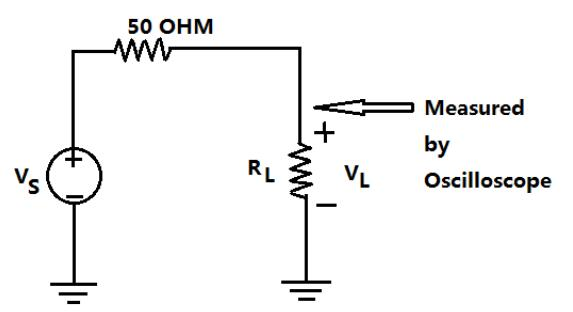
\includegraphics[width=.6\textwidth]{Figure1.jpg}
  \caption{Thevenin equivalent of a circuit}
  \label{img} 
\end{figure}
%---------------------------------

When the load $R_L$ is 50 $\Omega$ , according to voltage division, we know that the V$_L$ measured will be 0.5$V_S$. In this case, we use the 50 OHM mode, in which the function generator produces voltage $V_S$ but displays voltage 0.5$V_S$. In that way, if we set 2$V_{ppk}$ for the function generator, the actual $V_S$ will be 4$V_{ppk}$ to make sure the load get a voltage of 2$V_{ppk}$.

In our lab measurements, the load resistance $R_L$ is very high--the input resistance of the oscilloscope is about 1 $M\Omega$. The $V_L$ measured across $R_L$ practically equals $V_S$. So we use High Z mode, in which the function generator produce voltage $V_S$ and displays $V_S$.

\subsection{The Rise Time and Fall Time of signals}

The Rise time is the interval between the moment of the time when the signal reaches its 10\% level and the moment of time when the signal reaches its 90/%

%---------------------------------
  \begin{figure}[H]
  \centering
  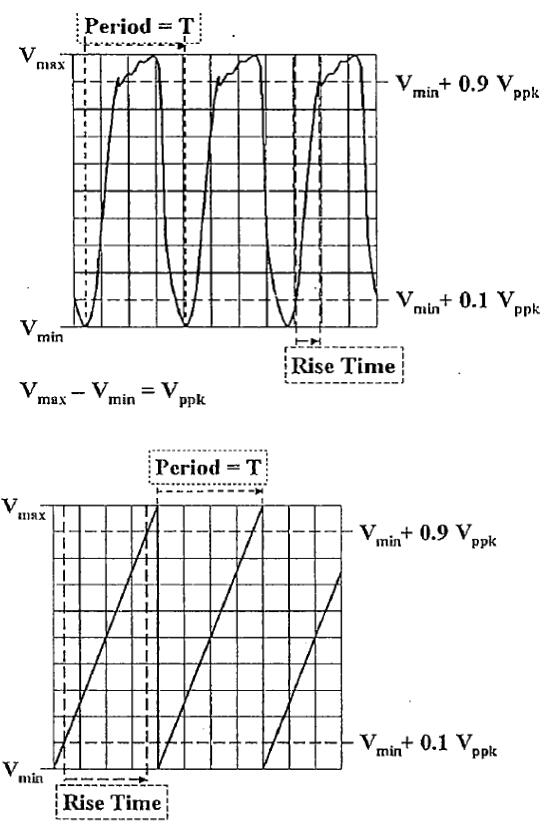
\includegraphics[width=.6\textwidth]{Figure2.jpg}
  \caption{Rise time of a sinusoidal like wave and a saw-tooth wave}
  \caption{$V_{RMS}$}
  \label{img} 
\end{figure}
%---------------------------------


Take the sinusoid wave as an example to calculate the rise time.

$$y=\frac{V_{ppk}}{2}\sin(2\pi ft)$$

$$V_{min}=\frac{-V_{ppk}}{2},V_{max}=\frac{V_{ppk}}{2}$$

$$Rise\ Time=\frac{\arcsin\left(\frac{V_{min}+0.9V_{ppk}}{0.5V_{ppk}}\right)-\arcsin\left(\frac{V_{min}+0.1V_{ppk}}{0.5V_{ppk}}\right)}{2\pi f}$$

\subsection{Fourier Series Representation of a Signal}

Fourier series is a way to represent a wave-like function as a combination of simply sine waves. It decomposed and period function into the sum of a (possibly infinite) set of simple oscillation functions.
Let $x(t)$ be a periodic signal with fundamental period $T_0$. It can be represent by the following synthesis equation,

$$x(t)=\sum_{k=-\infty}^{\infty}c_ke^{jk\omega_0t}, {\rm where} \omega_0=\frac{2\pi}{T_0}$$

The coefficients $c_k$ in the above equation can be calculated by the analysis equation,

$$C_k=\frac{1}{T_0}\int_0^{T_0}x(t)e^{-jk\omega_0t}dt,k=0,\pm 1,...$$

\subsection{Four ways to measure the amplitude of a sinusoid}

\begin{enumerate}

\item
$\rm V_{peak}=V_p=V_{pk}=V_0$ is the peak amplitude of the sinusoid measured in V or mV.
\item
$\rm V_{peak-to-peak}=V_{ppk}=V_{max}-V_{min}=2V_0$ is the value we often use in the lab to determine the overall size of the waveform. We have used it many times in the previous Labs.
\item
$\rm V_{RMS}$ is the Root-Mean-Square, or RMS amplitude of the sinusoid. The sinusoidal voltage $V=V_0\sin(\omega t+\theta)$ dissipates as much power in the load resistor as does the DC voltage equals to $V_{RMS}$
For any periodic function f(t) that has period T, the RMS amplitude is defined as
$$Amplitude,RMS=\sqrt{\frac{1}{T}\int_{t_0}^{t_0+T}f^2(t)dt}$$

In the case of sinusoid $f(t)=V_0\sin(\omega t+\theta)$,

$$V_{RMS}=\frac{V_0}{\sqrt{2}}=\frac{V_{peak}}{\sqrt{2}}=\frac{V_{ppk}}{2\sqrt{2}}$$
%---------------------------------
  \begin{figure}[H]
  \centering
  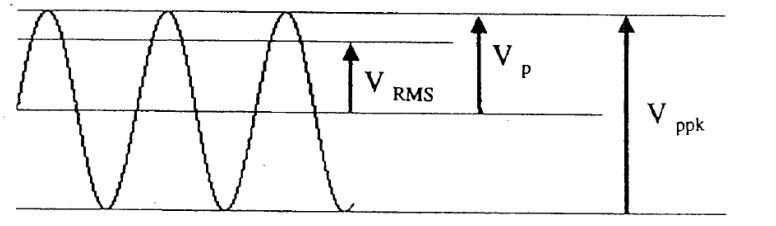
\includegraphics[width=.6\textwidth]{Figure3.jpg}
  \caption{$V_{RMS}$}
  \label{img} 
\end{figure}
%---------------------------------


\item
The above three ways all study the signal in time domain, plotted as voltage vs. time. In this Lab, we also need to study the frequency domain, when you measure their spectra displayed as amplitude vs. frequency. In frequency domain, the oscilloscope measures the amplitude of on a logarithmic scale, using decibels.

$$Amplitude\ in\ decibels(dBv)=20\log\left(\frac{Amplitude\ in\ V_{RMS}}{1V_{RMS}}\right)$$

Decibels are used to calculate ratios of two amplitudes on a logarithmic scale.

$$Ratio,in\ decibels(dB)=20\log\left(\frac{Amplitude\ of\ signal\ \sharp 2,RMS}{Amplitude\ of\ signal\ \sharp 1,RMS}\right)$$

\end{enumerate}

\section{In-Lab Procedure}
\subsubsection{Part 1}
\begin{enumerate}
\item
On the function generator, set a sine wave at 1 [kHz] and keep its amplitude at 3 [Vpp]. The load must be High-Z mode.

\item

Record the parameters on the datasheet. Fill the table with the data set on the function generator and displayed on the oscilloscope.

\item

Repeat the Step 2 with a sine wave at 1.5 [kHz] and 5 [Vpp] on the function generator. The load should remain High-Z mode.

\item

In post-report, calculate the rise time in theory and compare it with the values displayed on the oscilloscope.

\end{enumerate}

\subsubsection{Part 2}

\begin{enumerate}

\item

First, we set a sine wave and a square wave, respectively. The frequency is 1 [kHz] and the amplitude is 3 [Vpp].

\item

On the oscilloscope, set 1 [V/div] and 5 [ms/div].

\item

Push the “MATH” button and select “FFT” function.

\item

Push the “cursor” button and select “trace” mode to trace the spectrum.

\item

When the cursor reach a peak of the spectrum, record the Frequency in [kHz] and the Amplitude in [dBV].

\item

Set another sine wave and a square wave. The frequency is 2 [kHz] and the amplitude is 6 [Vpp]. Repeat the steps above.

\item

In post-report, we need to calculate the theoretical amplitude of sine wave in [dBV]. Besides, we need to calculate the Vpeak of each square wave measured in Part II. 
\end{enumerate}

\section{Results and Discussion}

\subsection{Part 1}



\begin{table}[H]

\begin{center}

\begin{tabular}{|c|c|c|}

\hline

 & Set on Function Generator & Measured with Oscilloscope \\

\hline

Amplitude in Vpp [V] 	&	3.000	&	3.000	\\

\hline

Frequency [kHz]			&	1.000	&	0.980	\\

\hline

Rise Time [$\mu$s]		&	295	&	300	\\

\hline

Amplitude in Vpp [V] 	&	5.000	&	5.080	\\

\hline

Frequency [kHz]			&	1.500	&	1.506	\\

\hline

Rise Time [$\mu$s]		&	197	&	196	\\

\hline

\end{tabular}

\caption{Rise Time Measurement.}

\label{tab-1}

\end{center}

\end{table}


The graph of the experiment is shown in the Figure 4.
%---------------------------------
  \begin{figure}[H]
  \centering
  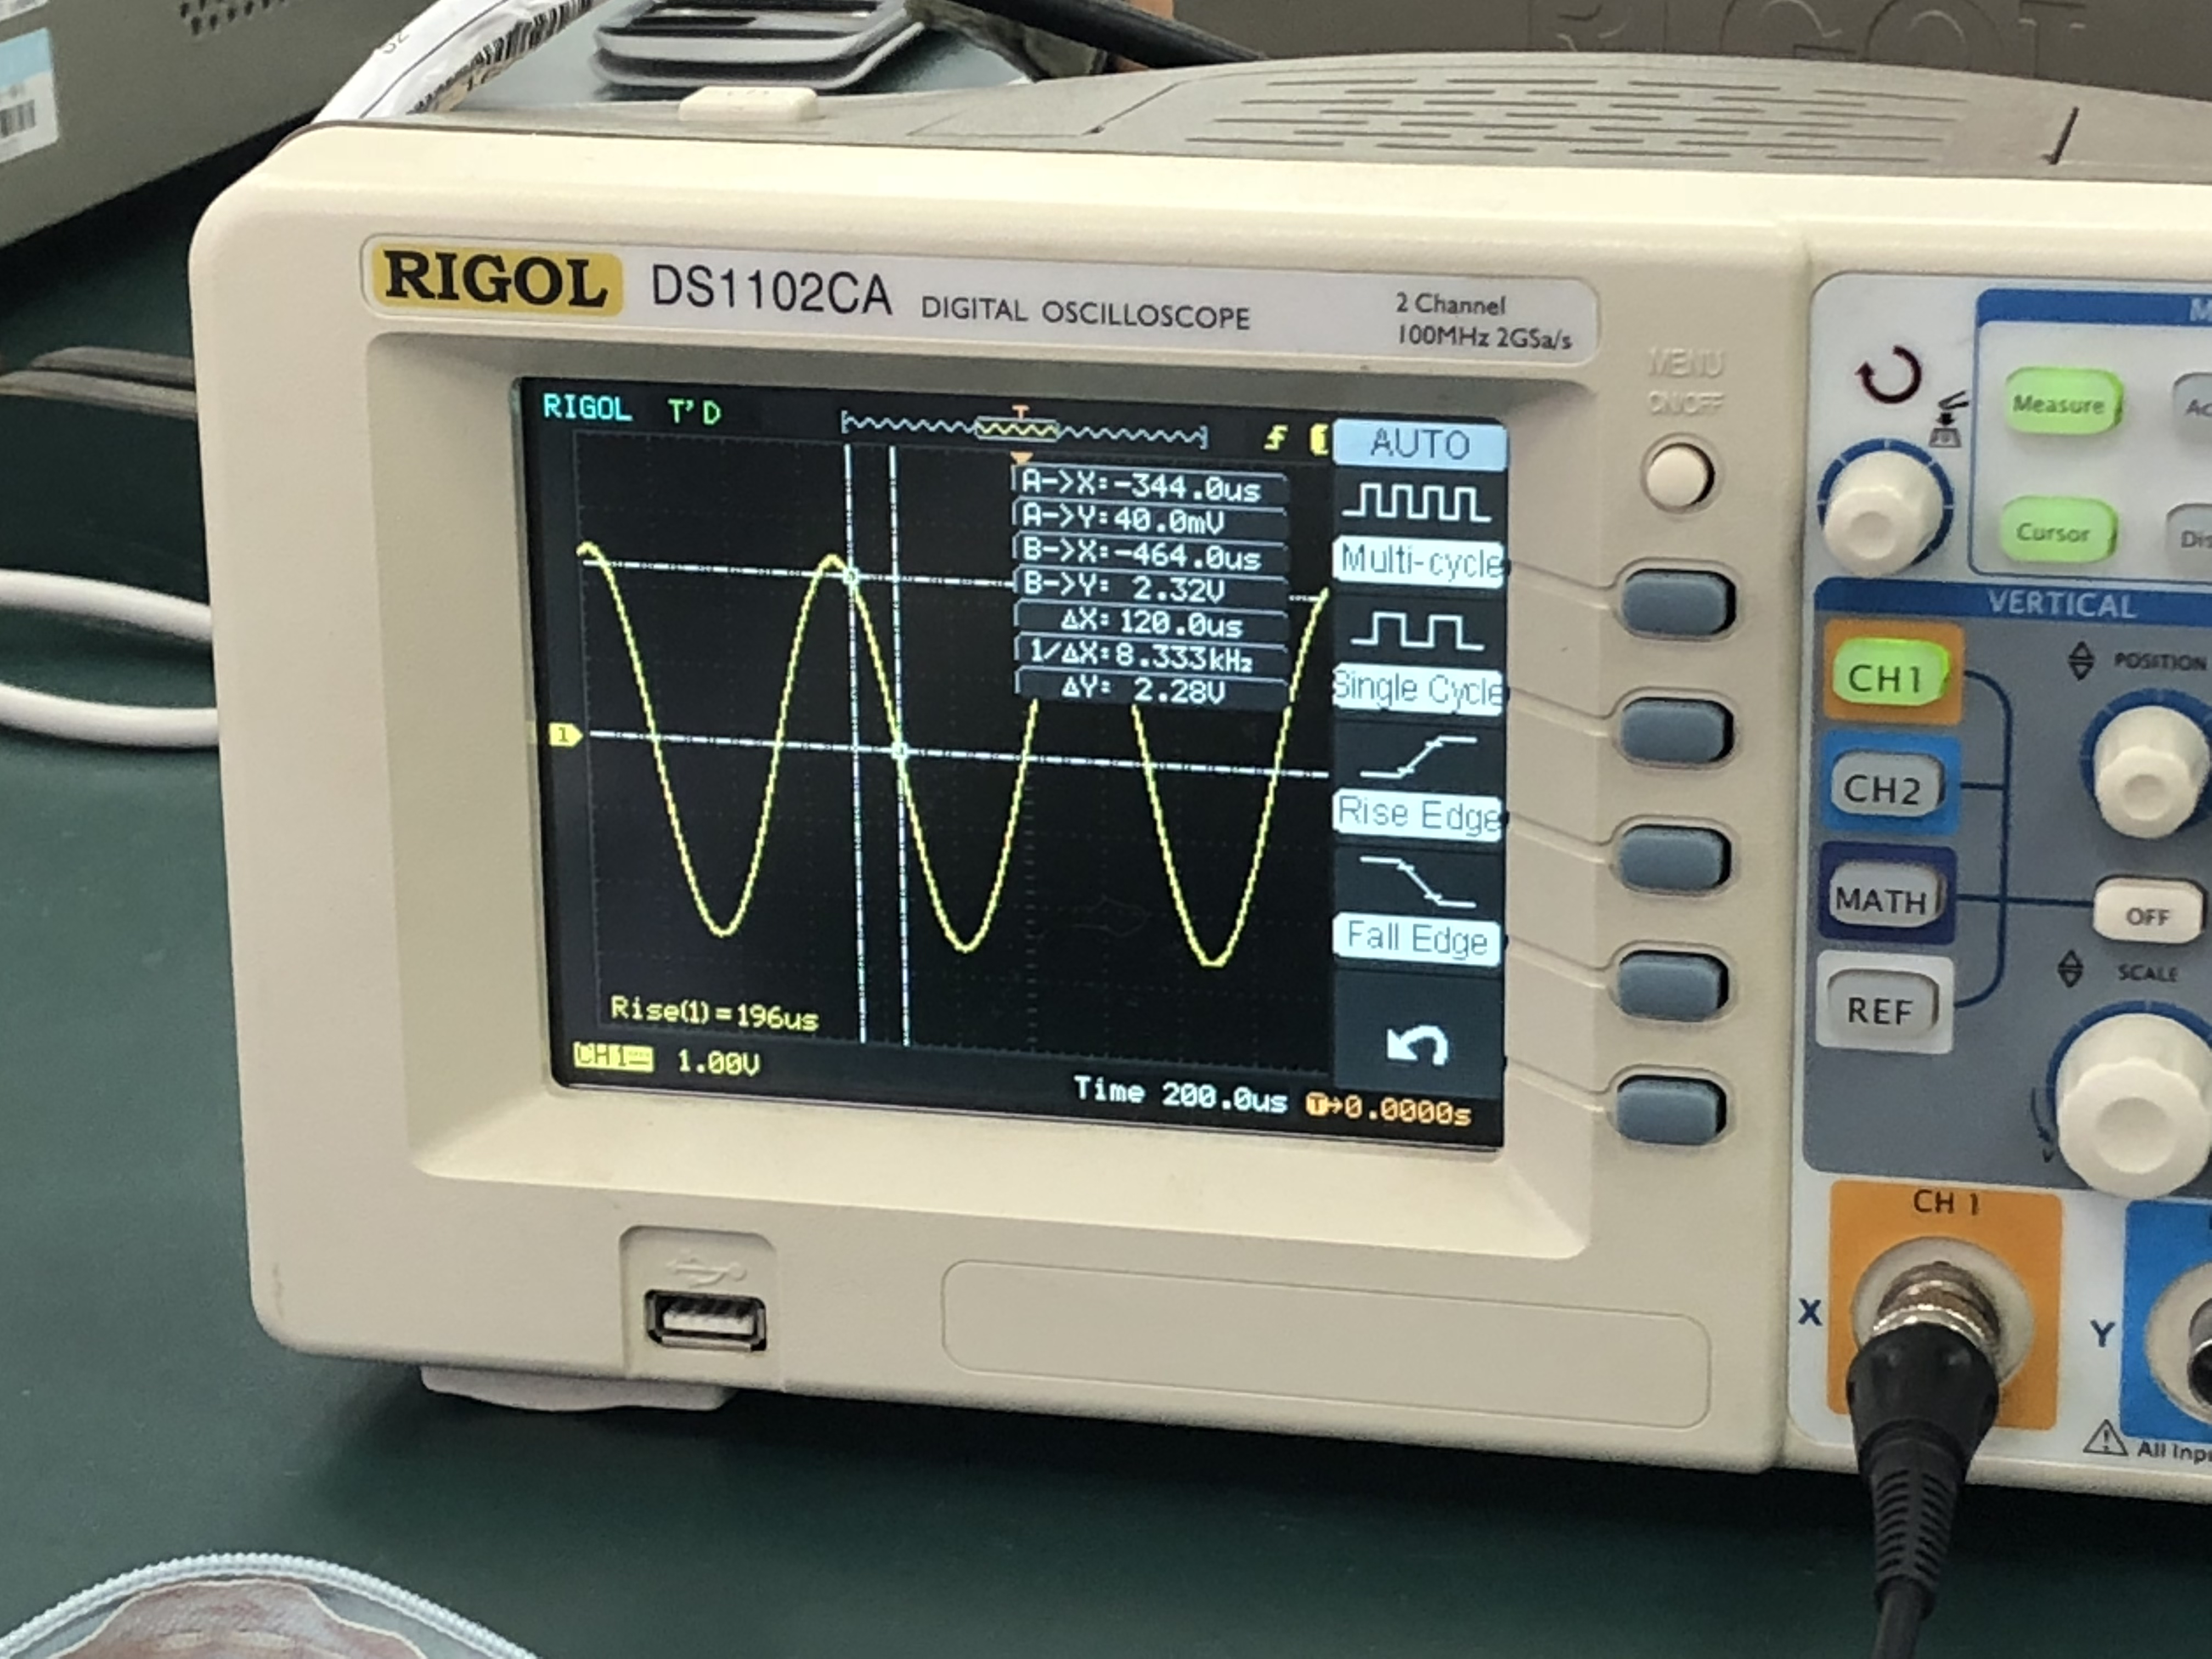
\includegraphics[width=.6\textwidth]{Figure4.jpg}
  \caption{Rise time measurement}
  \label{img} 
\end{figure}
%---------------------------------

For the 3V Vpp, the experimental rise time is

$$t=300\,\rm \mu s$$

Theoretically,

$$t=\frac{\arcsin\left(\frac{V_{min}+0.9V_{ppk}}{0.5V_{ppk}}\right)-\arcsin\left(\frac{V_{min}+0.1V_{ppk}}{0.5V_{ppk}}\right)}{2\pi f}=295\,\rm \mu s$$

The relative error is 
$$error = \frac{300-295}{295}\times 100\% = 1.69\%$$

For the 5V Vpp, the graph of the experiment is shown in the figure 5.
%---------------------------------
  \begin{figure}[H]
  \centering
  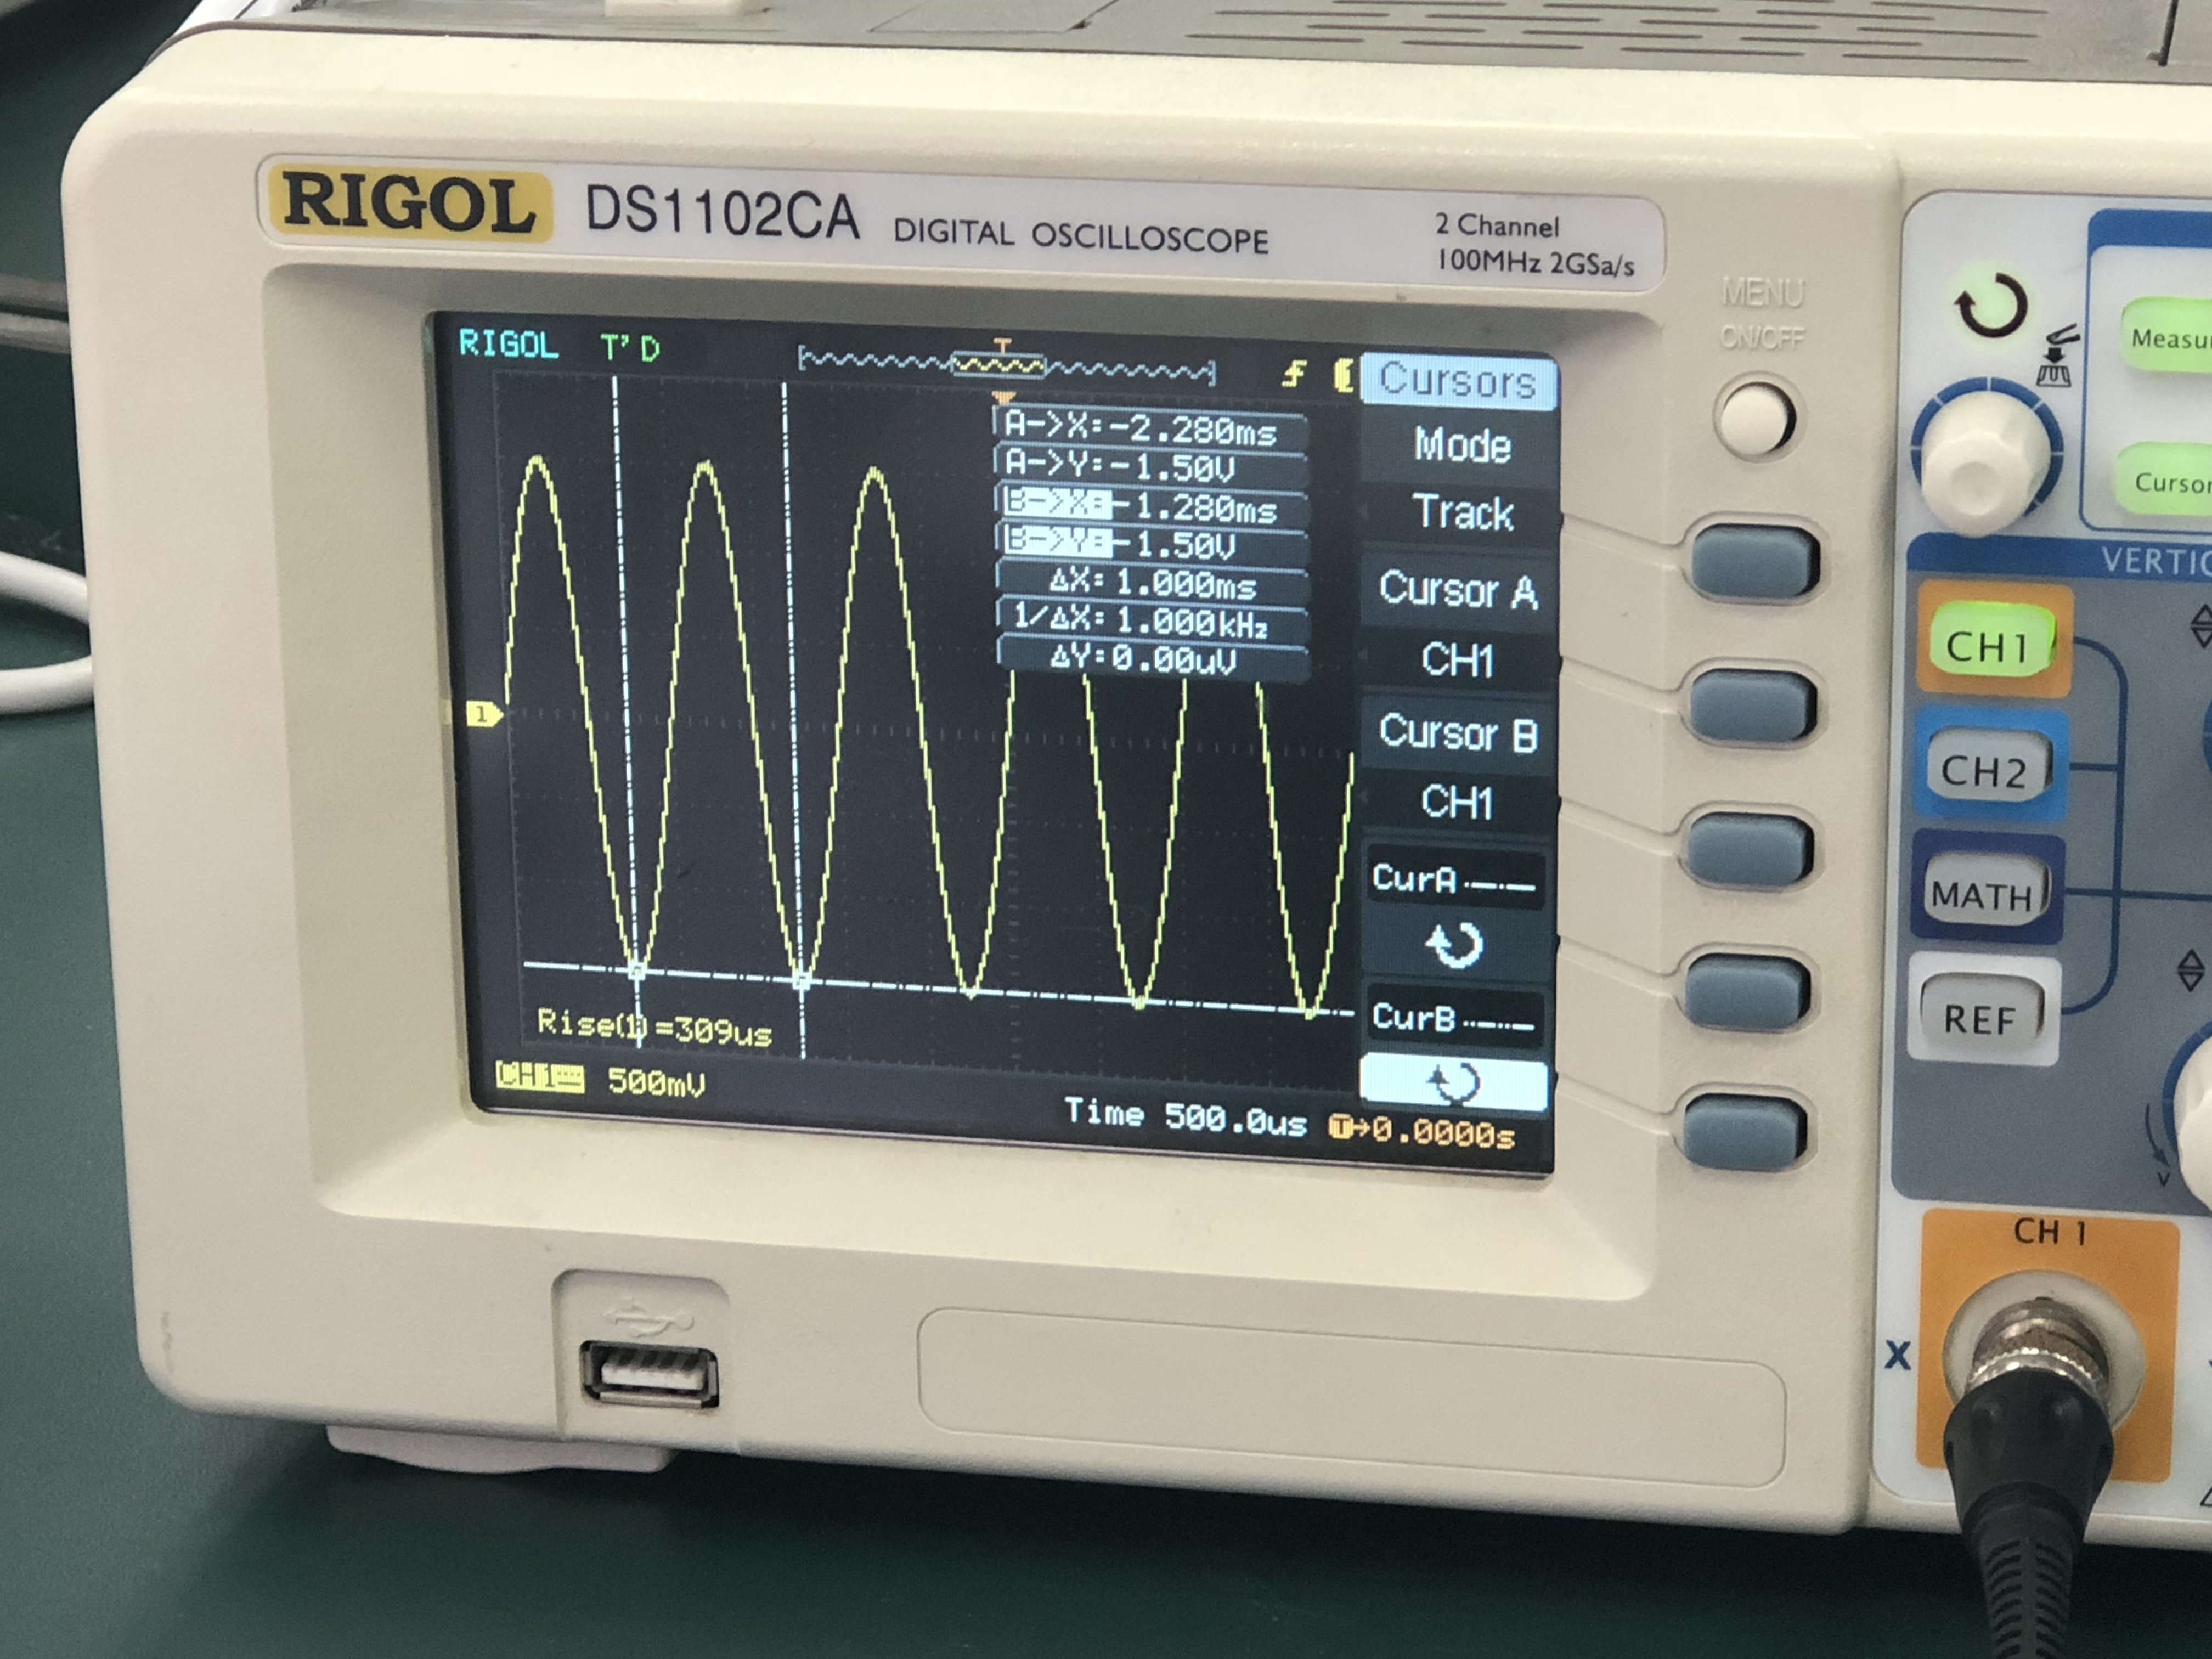
\includegraphics[width=.6\textwidth]{Figure5.jpg}
  \caption{Rise time measurement}
  \label{img} 
\end{figure}
%---------------------------------
The experimental rise time is

$$t=196\,\rm \mu s$$

Theoretically,

$$t=\frac{\arcsin\left(\frac{V_{min}+0.9V_{ppk}}{0.5V_{ppk}}\right)-\arcsin\left(\frac{V_{min}+0.1V_{ppk}}{0.5V_{ppk}}\right)}{2\pi f}=197\,\rm \mu s$$

The relative error is $1.6\%$\\
$$error = \frac{197-196}{196}\times 100\% = 0.51\%$$

We see that our error is very small which indicate the experiment is correct.
\subsection{Part 2}
\subsubsection{Set the wave at 3 [Vpp] 1 [kHz]}
%---------------------------------
  \begin{figure}[H]
  \centering
  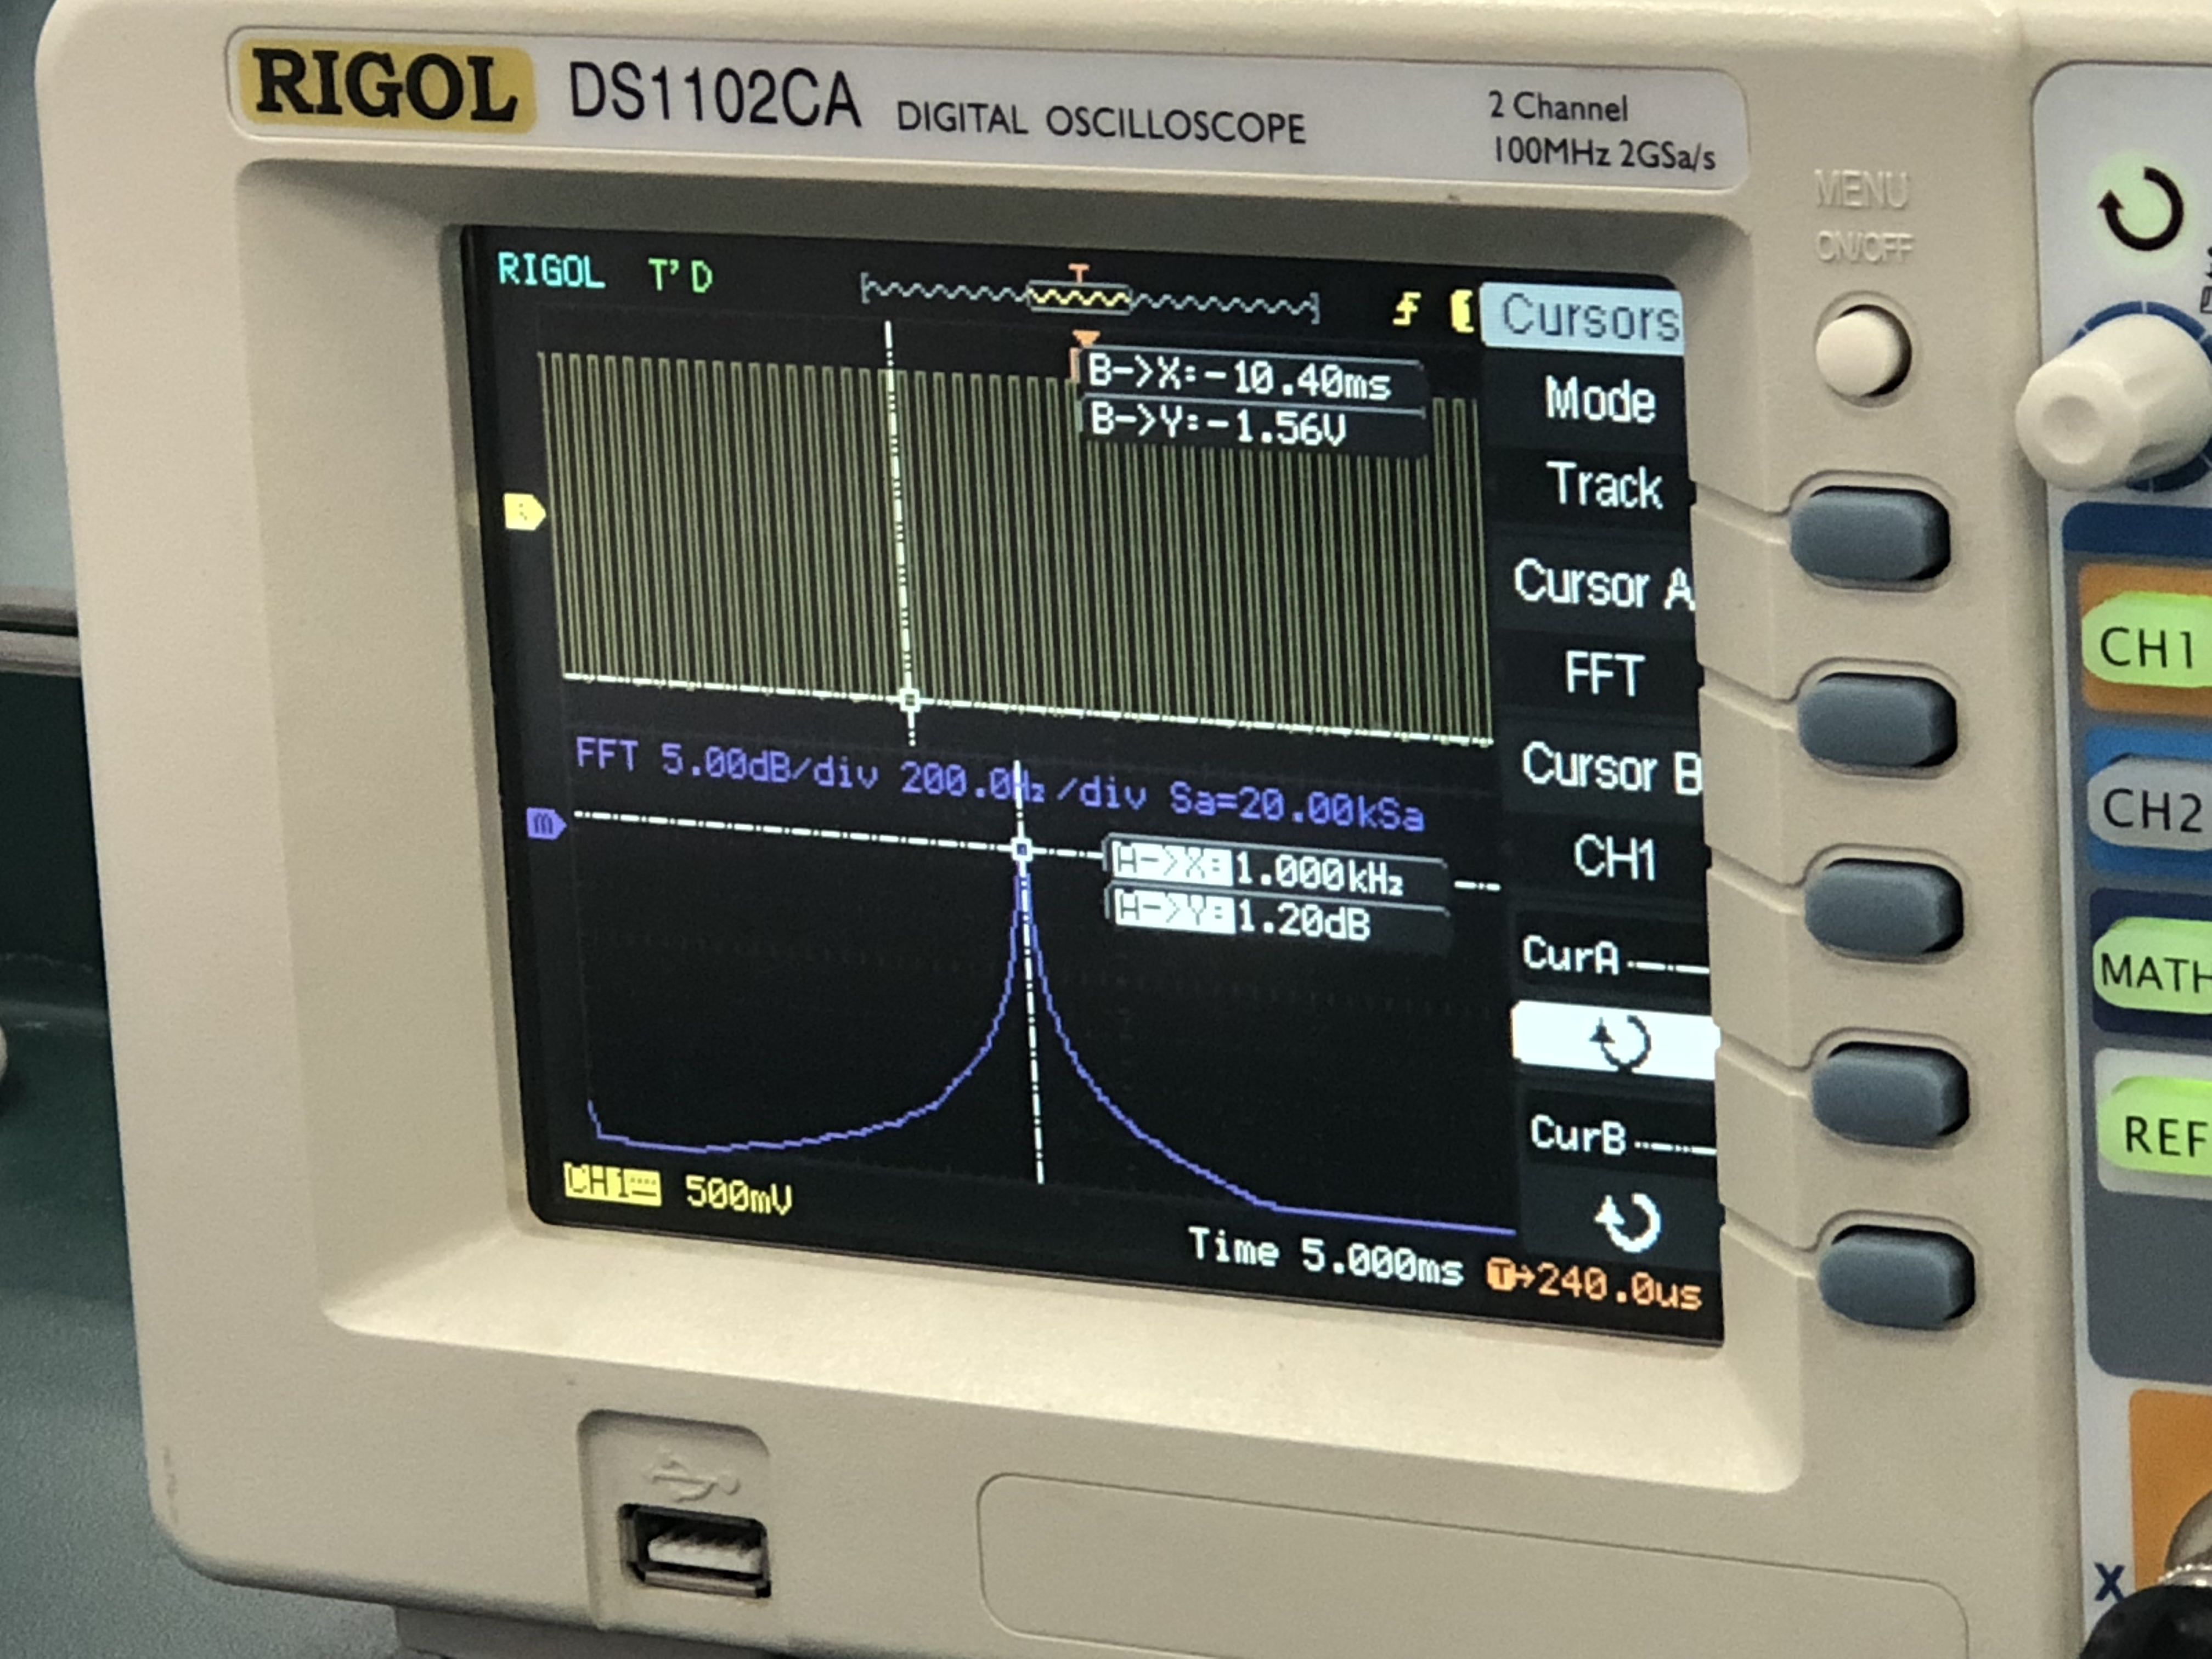
\includegraphics[width=.6\textwidth]{Figure7.jpg}
  \caption{FFT spectrum for Sine wave}
  \label{img} 
\end{figure}
%---------------------------------
\begin{table}[H]
\begin{center}
\begin{tabular}{|c|c|c|}
\hline
Peak & Frequency (measured) [kHz] & Amplitude (measured) [dBV] \\

\hline

$f_0$ &	1.000	&	-0.40	\\

\hline

\end{tabular}

\caption{FFT spectrum for Sine wave.}

\label{tab-2}

\end{center}

\end{table}
According to the experiment, the amplitude is 
$$A_{dBV}=-0.40$$

Theoretically,

$$A_{dBV}=20\log\left(\frac{A_{RMS}}{1V_{RMS}}\right)= 20\log (1.06)= 0.51$$

The relative error is $178\%$\\


Then we change the signal from sine wave to square wave. The following figure show what we've observed on the oscilliscope's screen.
%---------------------------------
  \begin{figure}[H]
  \centering
  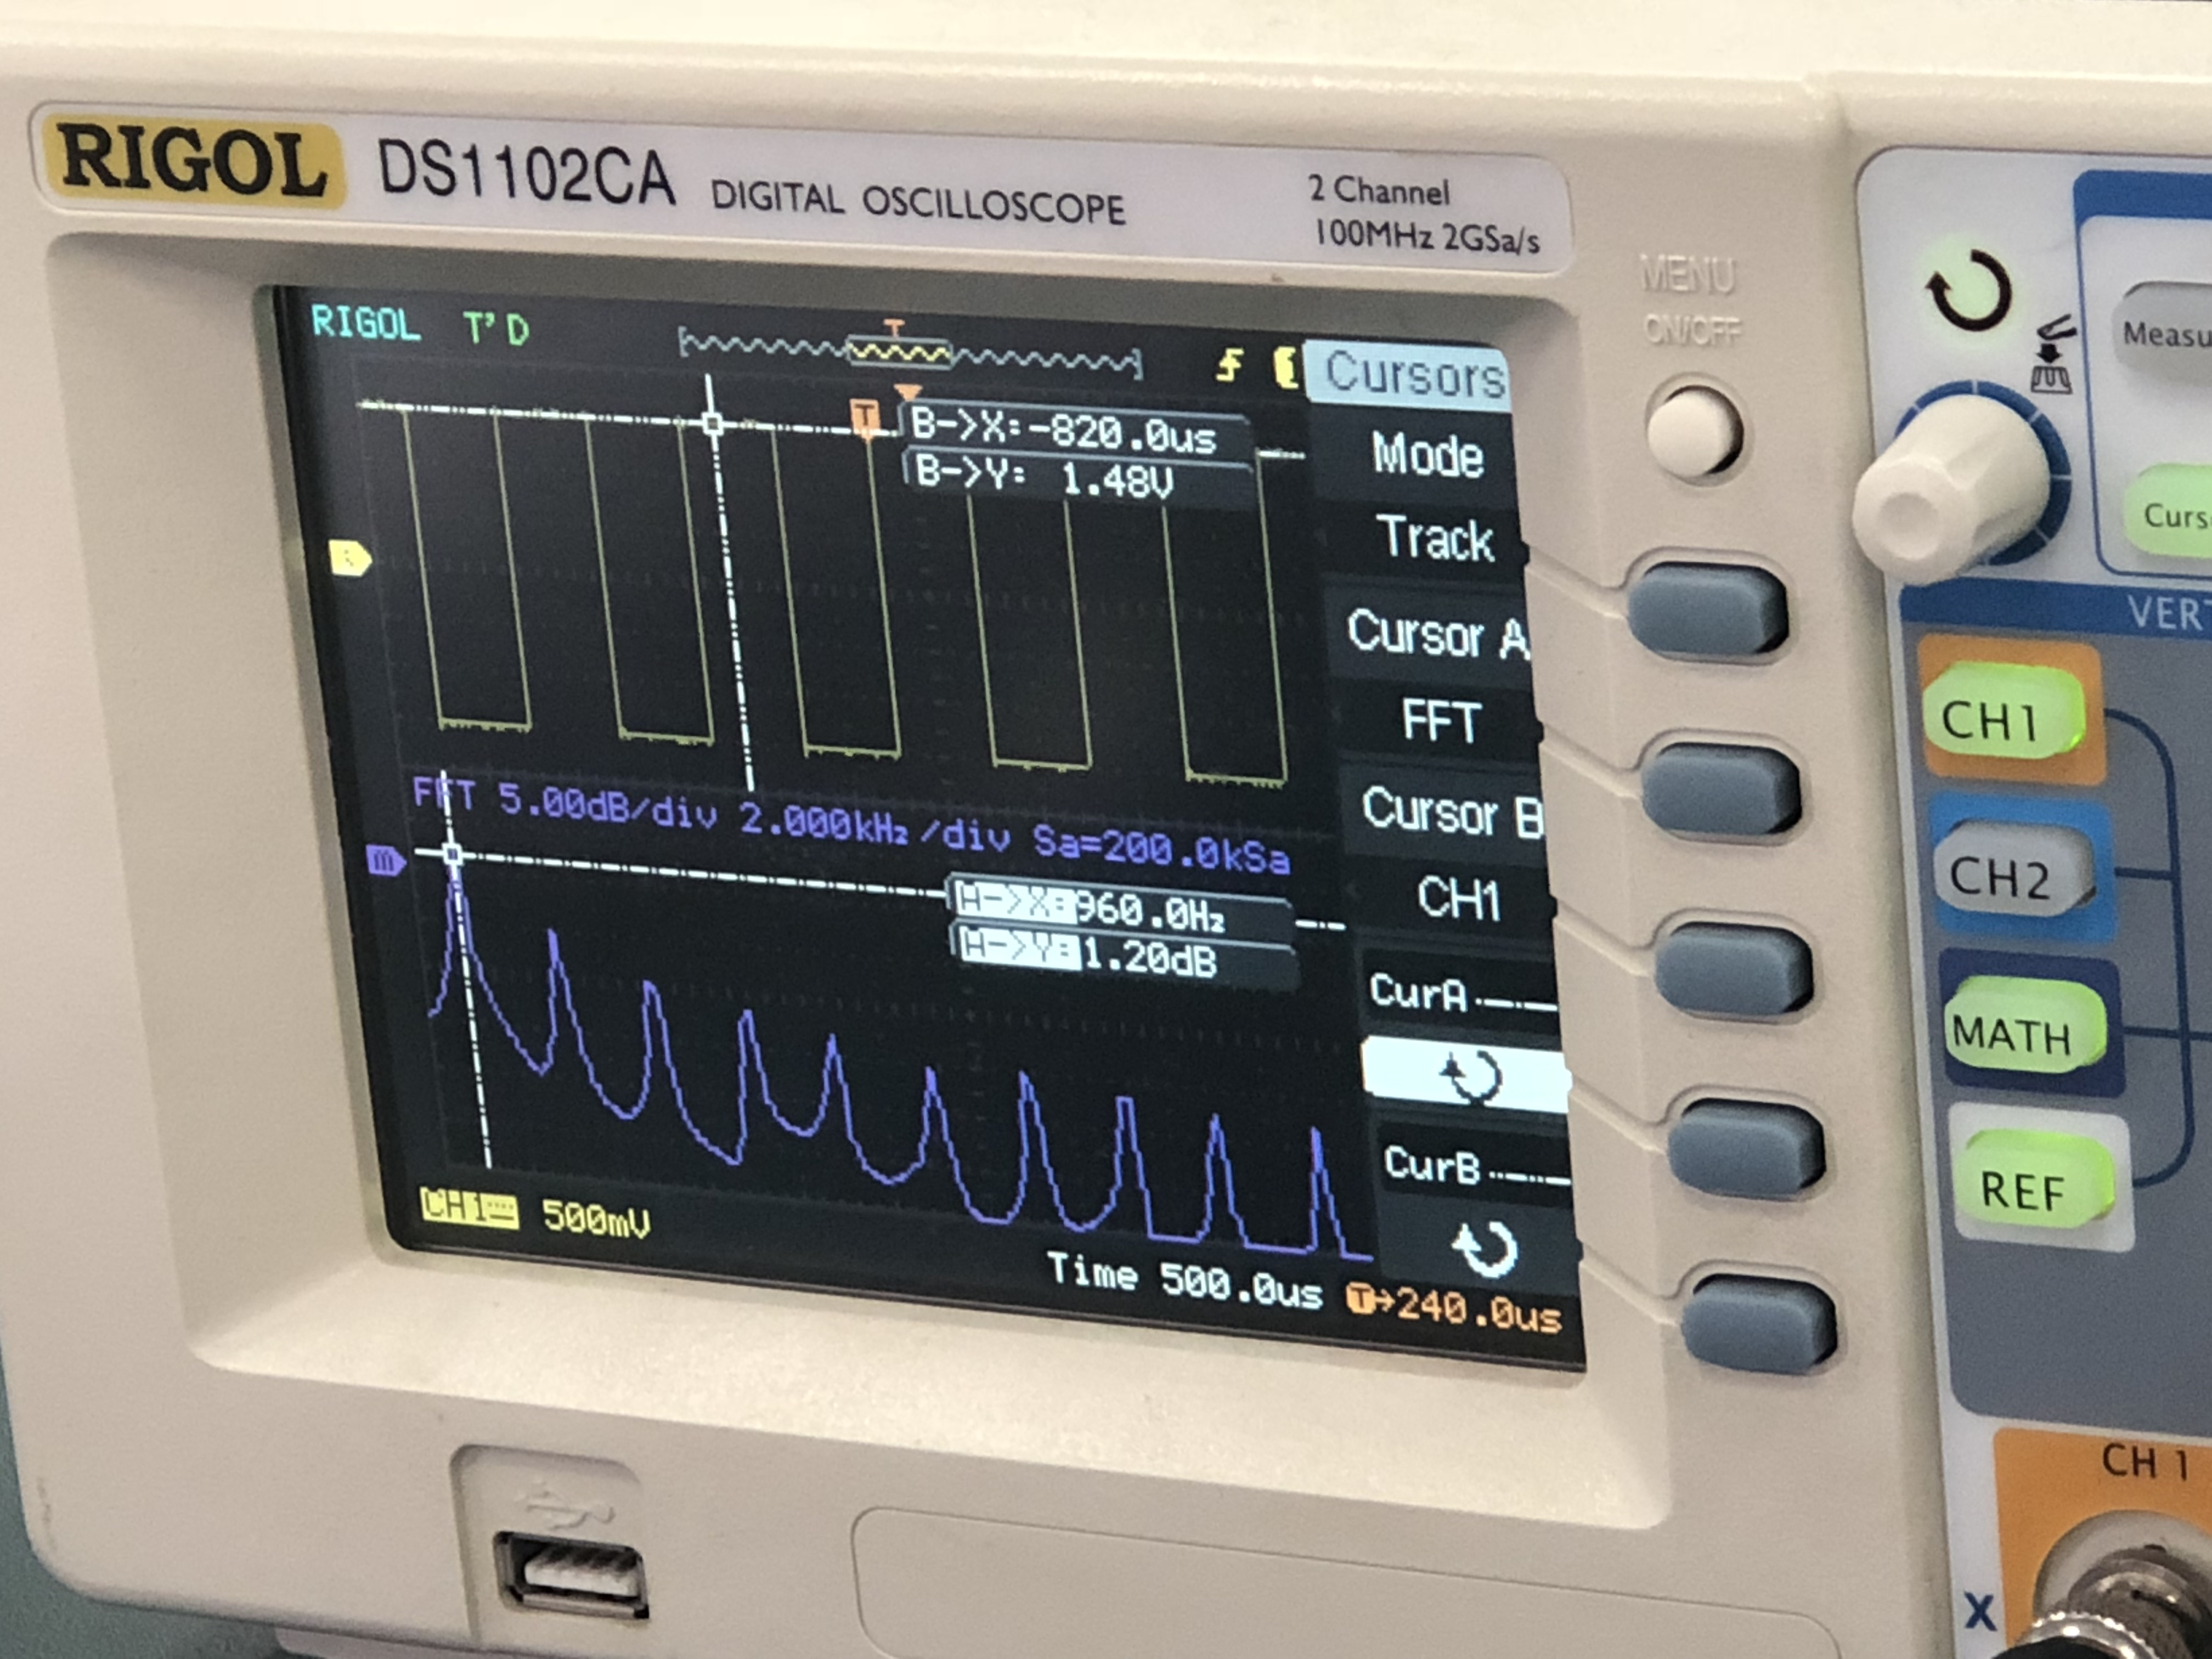
\includegraphics[width=.6\textwidth]{Figure6.jpg}
  \caption{FFT spectrum for square wave}
  \label{img} 
\end{figure}
%---------------------------------

\begin{table}[H]

\begin{center}

\begin{tabular}{|c|c|c|}

\hline

Peak & Frequency (measured) [kHz] & Amplitude (measured) [dBV] \\

\hline

$f_0$  &	0.960	&	1.200	\\

\hline

$3f_0$ &	3.040	&	-6.000	\\

\hline

$5f_0$ &	5.040	&	-10.00	\\

\hline

$7f_0$ &	7.120	&	-12.40	\\

\hline

$9f_0$ &	8.960	&	-14.00	\\
\hline
\end{tabular}
\caption{FFT spectrum for Square wave.}
\label{tab-3}
\end{center}
\end{table}

\subsubsection{Set the wave at 6 [Vpp] 2 [kHz]}

\begin{table}[H]

\begin{center}

\begin{tabular}{|c|c|c|}

\hline

Peak & Frequency (measured) [kHz] & Amplitude (measured) [dBV] \\

\hline

$f_0$ &	2.000	&	5.20	\\

\hline

\end{tabular}

\caption{FFT spectrum for Sine wave.}

\label{tab-4}

\end{center}

\end{table}

According to the experiment, the amplitude is

$$A_{dBV}= 5.20$$



Theoretically,



$$A_{dBV}=20\log\left(\frac{A_{RMS}}{1V_{RMS}}\right)=6.53$$



The relative error is 
$$error = \frac{6.53-5.20}{6.53}\times 100\%=20.3\%$$

Change the signal from sine wave to square wave and we obtain
\begin{table}[H]
\begin{center}
\begin{tabular}{|c|c|c|}
\hline
Peak & Frequency (measured) [kHz] & Amplitude (measured) [dBV] \\
\hline
$f_0$  &	2.000	&	6.00	\\
\hline
$3f_0$ &	6.080	&	-2.00	\\
\hline
$5f_0$ &	10.000	&	-4.40 	\\
\hline
$7f_0$ &	14.080	&	 -6.80	\\
\hline
$9f_0$ &	18.000	&	 -8.40	\\
\hline
\end{tabular}
\caption{FFT spectrum for Square wave.}
\label{tab-5}
\end{center}
\end{table}

\section{Conclusion}

In the lab, we learn how to define, calculate, and measure the amplitude of a sinusoidal signal. We also learn how to define, calculate, and measure the Rise Time and Fall Time of a signal. We learn how to observe FFT spectra of signal and measure their parameters with cursors.

Also, we have measured the waveforms and FFT spectra of various signals. We compared the theoretical results obtained in the Pre-Lab with the data we get from the experiment and find the error are relatively small which can be ignored. Therefore, this experiment can be considered successful.



\section{Reference}

Lab 4\_ AC LAB.




\end{document}